
\documentclass{article}
\usepackage{hyperref}
\usepackage[
    type={CC},
    modifier={by-nc-sa},
    version={3.0},
]{doclicense}
\usepackage[landscape]{geometry}
\usepackage{url}
\usepackage{multicol}
\usepackage{amsmath}
\usepackage{esint}
\usepackage{amsfonts}
\usepackage{tikz}
\usetikzlibrary{decorations.pathmorphing}
\usepackage{amsmath,amssymb}
\usepackage{ mathrsfs }

\usepackage{colortbl}
\usepackage{xcolor}
\usepackage{mathtools}
\usepackage{amsmath,amssymb}
\usepackage{enumitem}
\usepackage{empheq}

\makeatletter

\newcommand*\bigcdot{\mathpalette\bigcdot@{.5}}
\newcommand*\bigcdot@[2]{\mathbin{\vcenter{\hbox{\scalebox{#2}{$\m@th#1\bullet$}}}}}
\newcommand*\widefbox[1]{\fbox{\hspace{2em}#1\hspace{2em}}}

\makeatother

\title{MATH 215/255}
\usepackage[english]{babel}
\usepackage[utf8]{inputenc}

\renewcommand{\baselinestretch}{1.15}

\advance\topmargin-.8in
\advance\textheight3in
\advance\textwidth3in
\advance\oddsidemargin-1.5in
\advance\evensidemargin-1.5in
\parindent0pt
\parskip2pt
\newcommand{\hr}{\centerline{\rule{3.5in}{1pt}}}




%\colorbox[HTML]{e4e4e4}{\makebox[\textwidth-2\fboxsep][l]{texto}
\begin{document}

\begin{center}{\huge{\textbf{UBC MATH 215/255}}}\\
\end{center}
\begin{multicols*}{3}

\tikzstyle{mybox} = [draw=black, fill=white, very thick,
    rectangle, rounded corners, inner sep=10pt, inner ysep=10pt]
\tikzstyle{fancytitle} =[fill=black, text=white, font=\bfseries]

 
 %------------ Definitions ---------------
\begin{tikzpicture}
\node [mybox] (box){%
    \begin{minipage}{0.3\textwidth}
    \textbf{Some Common Equations}
    \hrule
    \vspace{.2cm}
    
    \large{
    	\begin{tabular}{||c|c||}
    	\hline
    $\frac{dy}{dx}=ky$ & $y(x)=Ce^{kx}$\\
    \hline
    $\frac{d^2y}{dx^2}=-k^2y$ & $y(x)=C_1\text{cos}(kx)+C_2\text{sin}(kx)$\\
    \hline
    $\frac{d^2y}{dx^2}=k^2y$ & $y(x)=C_1e^{kx}+C_2e^{-kx}$\\
    \hline
		\end{tabular}
	}
	\vspace{.3cm}
	\\
    \textbf{Definitions}
    \hrule
    \small{
    \begin{description}[font=\sffamily\bfseries, leftmargin=1.1cm, style=nextline]
  \item[ODE]  
  Equations where the derivatives are taken with respect to only one variable.
  \item[PDE]  
  Equations that depend on partial derivatives of several variables.
  \item[Order]
    The highest order derivative found in equation
  \item[Linear]
    $
a_n(x) \frac{d^n y}{dx^n} + 
a_{n-1}(x) \frac{d^{n-1} y}{dx^{n-1}} + 
\cdots
+
a_{0}(x) y = b(x) \notag
$

  \item[Coefficients]
  $a_n(x), a_{n-1}(x), ...  a_0$
  \item[Homogeneous]
$a_n(x) \frac{d^n y}{dx^n} + 
a_{n-1}(x) \frac{d^{n-1} y}{dx^{n-1}} + 
\cdots
+
a_{0}(x) y = 0 \notag
$
\item[Autonomous]
Equation does not depend on the independent variable
    
\end{description}
}
    \end{minipage}
};
%------------ Intro ---------------------
\node[fancytitle, right=10pt] at (box.north west) {Intro};
\end{tikzpicture}

%------------ Existence and Uniqueness ---------------
\begin{tikzpicture}
\node [mybox] (box){%
    \begin{minipage}{0.3\textwidth}
    \textbf{Picard's Theorem}
    \hrule
    \small{
    \vspace{.2cm}
   If $f(x,y)$ is continuous (as a function of two variables) and $\frac{\partial f}{\partial y}$ exists and is continuous near some $(x_0,y_0)$, then a solution to 
   \begin{equation*}
y' = f(x,y), \qquad y(x_0) = y_0,
\end{equation*}
exists (at least for some small interval of x's) and is unique.\\

}
    \end{minipage}
};
%------------ Existence and Uniqueness ---------------------
\node[fancytitle, right=10pt] at (box.north west) {Existence and Uniqueness};
\end{tikzpicture}



%-------------------Authorship-----------------------
\begin{center}
    \framebox{
    \parbox[t][.5cm]{6.5cm}{
    \addvspace{0.2cm} \centering 
    \footnotesize Compiled by Simon Ghyselincks 2021 
    } 
}
\end{center} 
s




%------------ First Order Equations ---------------
\begin{tikzpicture}
\node [mybox] (box){%
    \begin{minipage}{0.3\textwidth}
    \textbf{Integral Solutions}
    \hrule
    \small{
    \vspace{.2cm}
    \begin{equation}
y' = f(x) \notag
\end{equation}
\begin{equation*}
\int y'(x) \,dx = \int f(x) \,dx + C 
\end{equation*}
\begin{equation*}
y(x) = \int f(x) \,dx + C .
\end{equation*}
\textbf{For an IVP:  \ \ \ }  $y(x) = \int_{x_0}^x f(s) \,ds + y_0$
}
\\


\normalsize{
\textbf{Separable Equations}
}
    \hrule
    \vspace{.2cm}
\small{
\begin{equation*}
y' = f(x)g(y) \implies \frac{dy}{g(y)} = f(x) \,dx
\end{equation*}
\begin{equation*}
\int \frac{dy}{g(y)} = \int f(x) \,dx + C .
\end{equation*}
	}
	
	
	\normalsize{
\textbf{Linear Equations and Integrating Factor}
}
    \hrule
    \vspace{.2cm}
\normalsize{
\begin{equation*}
y' + p(x) y = f(x) \implies r(x) y' + r(x) p(x) y = r(x) f(x)
\end{equation*}
\begin{equation*}
\frac{d}{dx}r(x) = r(x)p(x) \implies r(x) = e^{\int p(x) \,dx}
\end{equation*}

\centering \textbf{General Form:}
\begin{equation*}
\boxed{
y  = e^{-\int p(x) \,dx} \left( \int e^{\int p(x) \,dx} f(x) \,dx + C \right) 
}
\end{equation*}

\centering \textbf{IVP Form:}
\begin{equation*}
\boxed{
y(x) = e^{-\int_{x_0}^x p(s)\, ds} \left( \int_{x_0}^x e^{\int_{x_0}^t p(s)\, ds}
f(t) \,dt + y_0 \right)
}
\end{equation*}
	}
	\normalsize{
\textbf{Substitution}
}
    \vspace{.1cm}
    \hrule
    \vspace{.1cm}
    
\normalsize{
    \begin{enumerate}
        \item $v=f(x,y)$ then find $y'$ in terms of $v',\,v,\,x$
        \item Rewrite original equation in terms of $v',\,v,\,x$
        \item Solve equation for $v$ and resubstitute $f(x,y)=v$
    \end{enumerate}
    \textbf{Bernoulli Equations:}\\
    \large {For $y' + p(x)y = q(x)y^n$ use $v=y^{1-n}$}
}
	

    \end{minipage}
};
%------------ 1st ODEs ---------------------
\node[fancytitle, right=10pt] at (box.north west) {First Order Equations};
\end{tikzpicture}



 %------------ Autonomous Equations ---------------
\begin{tikzpicture}
\node [mybox] (box){%
    \begin{minipage}{0.3\textwidth}
    \begin{equation*}
        \large{\boxed{
        y' = f(y)
        }}
    \end{equation*}

    \textbf{Definitions}
    \hrule
    \small{
    \begin{description}[font=\sffamily\bfseries]
  \item[Equilibrium Solution]  
  Constant solutions where $y' = 0$
  \item[Critical points]  
  Points where $f(y) = 0$
  \item[Stable]
    A critical point that attracts neighboring positions
  \item[Unstable]
  A critical point that is not stable
  \item[Phase Diagram:]
 \end{description}
  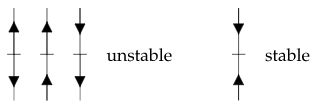
\includegraphics[width=6.5cm]{images/phase points.png}
  }
    \end{minipage}
};
%------------ Autonomous Equations ---------------------
\node[fancytitle, right=10pt] at (box.north west) {Autonomous Equations};
\end{tikzpicture}



 %------------ Euler's Method ---------------
\begin{tikzpicture}
\node [mybox] (box){%
    \begin{minipage}{0.3\textwidth}
    \begin{equation*}
        \large{\boxed{
        y'=f(x, y), \,\,y(x_0)=y_0
        }}
    \end{equation*}

    \textbf{Description}
    \hrule
    \vspace{.2cm}
    \large{
    
    Make successive approximations as follows:
    \begin{tabular}{||c|c||}
    \hline
     $x_{n+1}= x_n + \Delta x$ &  $y_{n+1}= y_n + f(x_n,y_n)\Delta x $\\
    \hline
    \end{tabular}
    }


    \end{minipage}
};
%------------ Autonomous Equations ---------------------
\node[fancytitle, right=10pt] at (box.north west) {Euler's Method};
\end{tikzpicture}


\end{multicols*}

%------------ CC License -----------------------------
\doclicenseThis

\linespread{1.3}

\begin{multicols*}{3}
\tikzstyle{mybox} = [draw=black, fill=white, very thick,
    rectangle, rounded corners, inner sep=10pt, inner ysep=10pt]
\tikzstyle{fancytitle} =[fill=black, text=white, font=\bfseries]


%--------------New Pages --------------------
\newpage
%--------------New Pages --------------------



%------------ Existence, Uniqueness, Superposition ---------------
\begin{tikzpicture}
\node [mybox] (box){%
    \begin{minipage}{0.3\textwidth}
\textbf{Superposition}
    \hrule
    \normalsize{
    \vspace{.2cm}
    Suppose $y_1$ and $y_2$ are two solutions of the homogeneous equation 
    \begin{equation*}
       y'' + p(x)y' + q(x)y = 0 
    \end{equation*}
    Then $y(x) = C_1 y_1(x) + C_2 y_2(x)$ also is a solution\\
    \hrule
    \vspace{.2cm}
    If $p$ and $q$ are continuous functions and $y_1$ and $y_2$ are linearly independent, then we can also say that it is the general (unique) solution.
    \\
    
    \textbf{Existence and Uniqueness}
    \hrule
    \vspace{.2cm}
    Suppose $p,q,f$ are continuous functions on some interval $I$, $a$ is within $I$, and $a,b_0,b_1$ are constants:
    \begin{equation*}
        y'' + p(x) y' + q(x) y = f(x) ,
    \end{equation*}
    has exactly one unique solution $y(x)$ defined on the same interval $I$ with initial conditions:
        \begin{equation*}
y(a) = b_0 \ \ \ \ y'(a) = b_1 
\end{equation*}

}
\end{minipage}
};
%------------ 2nd Order Existence, Uniqueness, Superposition ---------------------
\node[fancytitle, right=10pt] at (box.north west) {Superposition, Existence, Uniqueness};
\end{tikzpicture}

%------------ Second Order Equations ---------------
\begin{tikzpicture}
\node [mybox] (box){%
    \begin{minipage}{0.3\textwidth}
    \textbf{Constant Coefficient}
    \hrule
    \small{
    \vspace{.2cm}
\begin{equation*}
\text{For: }a y'' + b y' + c y = 0
\end{equation*}
Try the substitution $y=e^{rx}$, then
\begin{equation*}
e^{rx}(ar^2+br+c) = 0
\end{equation*}
where $ar^2+br+c = 0$ is the characteristic equation.\\  
Solve for $r$ using quadratic formula.

\vspace{.2 cm}

    \begin{tabular}{||c|c||}
    \hline
    \textbf{$r$ values} & \textbf{General Solution}\\
    \hline
    \hline
    $r_1 \neq r_2$: & $y = C_1 e^{r_1 x} + C_2 e^{r_2 x}$\\
    \hline
    $r_1 = r_2$: & $y = (C_1 + C_2 x)\, e^{r_1 x}$\\
    \hline
    $r\notin \mathbb{R}, r=\alpha+\beta i$: & $y=C_1e^{\alpha x}\text{cos}(\beta x)+C_2e^{\alpha x}\text{sin}(\beta x)$\\
    \hline
		\end{tabular}
	


}
    \end{minipage}
};
%------------ 2nd Order ODE ---------------------
\node[fancytitle, right=10pt] at (box.north west) {Second Order Linear Homogeneous};
\end{tikzpicture}

%------------ 2nd Order Applications ---------------
\begin{tikzpicture}
\node [mybox] (box){%
    \begin{minipage}{0.3\textwidth}
    \textbf{Mechanical Vibrations}
    \hrule
    \small{
    \vspace{.2cm}
    
    \begin{equation}
mx''+cx'+kx=F(t) \notag
\end{equation}


\begin{tabular}{||c|c||}
    	\hline
    \textbf{Forced} if $F \not \equiv 0$ & \textbf{Damped} if $c > 0$  \\
    \hline
   \textbf{Unforced/Free} if $F \equiv 0$ & \textbf{Undamped} if $c = 0$\\
   \hline
    		\end{tabular}
}
\\

\small{
\textbf{Undamped}
    \hrule
    \vspace{.2cm}

%Case 1 -----------------------------

\begin{equation*}
mx'' + kx = 0 \implies x'' + \omega_0^2 x = 0 ,\,\,\omega_0 = \sqrt{\frac{k}{m}}
\end{equation*}
\begin{equation*}
x(t) = A \cos (\omega_0 t) + B \sin (\omega_0 t) = C \cos ( \omega_0 t - \gamma )
\end{equation*}
\begin{center}
\boxed{x(t) = C \cos ( \omega_0 t - \gamma ), \ \
C= \sqrt{A^2 + B^2}, \ \
\tan (\gamma) = \frac{B}{A}}\\
\end{center}
\vspace{.2cm}

\textbf{Damped:}
    \hrule
\begin{equation*}
x_c =
\begin{cases}
C_1 e^{r_1 t} + C_2 e^{r_2 t} & \text{if } \; c^2 > 4km , \\
C_1 e^{-p t} + C_2 t e^{-p t} & \text{if } \; c^2 = 4km , \\
e^{-p t} \bigl( C_1 \cos (\omega_1 t) + C_2 \sin (\omega_1 t) \bigr) &
\text{if } \; c^2 < 4km ,
\end{cases}
\end{equation*}
%Case 2 -----------------------------
\textbf{Overdamping:}
}
    \hrule
    \vspace{.2cm}
\small{


\centering\boxed{x(t) = C_1 e^{r_1 t} + C_2 e^{r_2 t}}
\vspace{.2cm}

%Case 3 -----------------------------
\textbf{Underdamping:}
}
    \hrule
    \vspace{.2cm}
\small{


\begin{equation*}
r = p \pm \sqrt{p^2 - \omega_0^2}= \ \   p\pm \omega_1i\ \  \\  
\end{equation*}
\begin{equation*}
x(t) = e^{-pt} \bigl( A \cos (\omega_1 t) + B \sin (\omega_1 t) \bigr)
\end{equation*}
\centering\boxed{x(t) = C e^{-pt} \cos ( \omega_1 t - \gamma )}\\
	}
	
	\vspace{.5cm}
	\textbf{RLC Circuit}
	\vspace{.1cm}
	\hrule
	\begin{center}
	    \boxed{L I''(t) + R I'(t) + \frac{1}{C} I(t) = E'(t)}
	\end{center}
	
		\vspace{.3cm}
	\textbf{Pendulum Behavior}
	\vspace{.1cm}
	\hrule
	\begin{center}
	\boxed{\theta'' + \frac{g}{L} \sin \theta = 0}
	\end{center}
	
    \end{minipage}
};
%------------ 2nd Order Applications ---------------------
\node[fancytitle, right=10pt] at (box.north west) {2nd Order Applications};
\end{tikzpicture}

%------------ Second Order Non-homo ---------------
\begin{tikzpicture}
\node [mybox] (box){%
    \begin{minipage}{0.3\textwidth}
    \textbf{Constant Coefficient}
    \hrule
    \small{
    \vspace{.2cm}
\begin{equation}
\text{For: }a y'' + b y' + c y = g(x) \tag{1}
\end{equation}
If $y_p$ is a particular solution to the equation (1), and $y_c$ is the complimentary solution to the associated homogeneous equation, then the general solution to (1) is:
\begin{equation*}
    y=y_p+y_c
\end{equation*}
}
\textbf{Method of Undetermined Coefficients}
    \hrule
    \vspace{.2cm}
    If $g(x)$ above has finitely many linearly independent derivatives, then we can "guess" the proper solution:        $$y_p = A_1P_1(x)+A_2P_2(x)+ ... A_nP_n(x)$$

    
\textbf{Variation of Parameters}
    \hrule
    \vspace{.2cm}
    
    For $y_c = y_1 + y_2$ and $y'' + f(x)y' + h(x)y = g(x)$ \textbf{note that the factor of $y''$ is 1}, to find the particular solution $y_p$ 
    \begin{center}
      \boxed{
        y_p = u_1 y_1 + u_2 y_2
    }\\ 
    \vspace{.2cm}
    
    
    $\mathcal{W}(y_1,y_2)=\det \begin{vmatrix}
 y_1  & y_2 \\ 
 y_1' & y_2' 
\end{vmatrix} = y_1y_2'-y_2y_1'$
\\
\vspace{.2cm}
\boxed{
       u_1 = -\int \frac{y_2g(x)}{\mathcal{W}(y_1,y_2)} \ \ \ \ \  u_2 =\int \frac{y_1g(x)}{\mathcal{W}(y_1,y_2)}
    }

\end{center}
    \end{minipage}
};
%------------ 2nd Order Nonhomo ---------------------
\node[fancytitle, right=10pt] at (box.north west) {Second Order Linear Nonhomogenous};
\end{tikzpicture}

%------------ Forced Oscillations Pt 1 ---------------
\begin{tikzpicture}
\node [mybox] (box){%
    \begin{minipage}{0.3\textwidth}
    \begin{center}
    \boxed{mx'' + kx = F_0 \cos (\omega t)}
    \vspace{.2cm}\\
Solving for the case where $\omega \neq \omega_0$: 
    \begin{equation*}
\boxed{
x = C_1 \cos (\omega_0 t) + C_2 \sin (\omega_0 t) +
\frac{F_0}{m(\omega_0^2 - \omega^2)} \cos (\omega t)
}
\end{equation*}
    \hrule
    \vspace{.2cm}
    Solving for the case where $\omega = \omega_0$: 
    \begin{equation*}
\boxed{x = C_1 \cos (\omega t) + C_2 \sin (\omega t)
+ \frac{F_0}{2m\omega} \, t \sin (\omega t) }
\end{equation*}
\end{center}

    \end{minipage}
};
%------------ Forced Oscillations Part 1 ---------------------
\node[fancytitle, right=10pt] at (box.north west) {Undamped Forced Oscillations};
\end{tikzpicture}


%Page Break---------------------------------


%------------ Forced Oscillations Part 2 ---------------
\begin{tikzpicture}
\node [mybox] (box){%
    \begin{minipage}{0.3\textwidth}
    \begin{center}
    \boxed{mx'' + cx' + kx = F_0 \cos (\omega t)}
\end{center}
\begin{equation*}
x_c =
\begin{cases}
C_1 e^{r_1 t} + C_2 e^{r_2 t} & \text{if } \; c^2 > 4km , \\
C_1 e^{-p t} + C_2 t e^{-p t} & \text{if } \; c^2 = 4km , \\
e^{-p t} \bigl( C_1 \cos (\omega_1 t) + C_2 \sin (\omega_1 t) \bigr) &
\text{if } \; c^2 < 4km ,
\end{cases}
\end{equation*}


    \textbf{Particular Solution}
    \hrule
\begin{equation*}
\begin{split}
x_p = 
\frac{(\omega_0^2-\omega^2) F_0}
{m{(2\omega p)}^2+m{(\omega_0^2-\omega^2)}^2} \cos (\omega t)\\
+ \frac{2 \omega p F_0}
{m{(2\omega p)}^2+m{(\omega_0^2-\omega^2)}^2} \sin (\omega t) 
\end{split}
\end{equation*}

\begin{equation*}
\boxed{
x_p = 
\frac{F_0}{m \sqrt{{(2\omega p)}^2+{(\omega_0^2-\omega^2)}^2}} 
\cos ( \omega t - \gamma )
}
\end{equation*}



For all $x_c$, the value tends to zero as $t \rightarrow \infty$ because of damping.  The particular solution becomes dominant over time, with maximum amplitude for the particular solution being reached at:

\begin{equation*}
\boxed{
\omega = \sqrt{\omega_0^2 - 2p^2}
}
\end{equation*}
If $\omega_0^2 - 2p^2 < 0$ then there is no maximum resonance 



    \end{minipage}
};



%------------ Forced Oscillations Part 2 ---------------------
\node[fancytitle, right=10pt] at (box.north west) {Damped Forced Oscillations};
\end{tikzpicture}

%------------ Systems Of ODEs ---------------
\begin{tikzpicture}
\node [mybox] (box){%
    \begin{minipage}{0.3\textwidth}
    \textbf{Converting 2nd Order to 1st Order System}
    \hrule
    \vspace{.2cm}
    \begin{equation*}
        y'' + f(x)y' + g(x)y = h(x)
    \end{equation*}
    \begin{equation*}
        x_1 = y , \ \ x_2 = y' 
    \end{equation*}
        \begin{equation*}
        \begin{bmatrix}
        x_1' \\ x_2'
    \end{bmatrix}
    =
    \begin{bmatrix}
    0 & 1 \\ 
    -g(x) & -f(x) 
    \end{bmatrix}
        \begin{bmatrix}
        x_1 \\ x_2
    \end{bmatrix}
    +
    \begin{bmatrix}
        0 \\ h(x)
    \end{bmatrix}
    \end{equation*}
    
    More generally, $\vec{x'}(t)=A(t)\Vec{x}(t)+\vec{k}(t)$


    \end{minipage}
};
%------------ Systems Of ODEs ---------------------
\node[fancytitle, right=10pt] at (box.north west) {Systems Of ODEs};
\end{tikzpicture}

%------------ Eigenvalue Analysis ---------------
\begin{tikzpicture}
\node [mybox] (box){%
    \begin{minipage}{0.3\textwidth}
    \textbf{Eigenvalues and vectors}
    \hrule
    \vspace{.2cm}
    Find the eigenvalues first then solve for vectors:
    \begin{equation*}
        \det (A-\lambda I) = 0
    \end{equation*}
    \begin{equation*}
    (A-\lambda I) \vec{v} = \vec{0} ,
    \end{equation*}
    \begin{equation*}
    \boxed{
    \vec{x} = c_1 \vec{v}_1 e^{\lambda_1 t} +
    c_2 \vec{v}_2 e^{\lambda_2 t} + \cdots +
    c_n \vec{v}_n e^{\lambda_n t}
    }
    \end{equation*}
    \begin{equation*}
        \vec{x}(t) = \underbrace{
        \bigl[\, \vec{v}_1 e^{\lambda_1 t} \quad \vec{v}_2 e^{\lambda_2 t}
        \quad \cdots \quad \vec{v}_n e^{\lambda_n t} \,\bigr]}
            _\textrm{Fundamental Matrix} 
        \times \underbrace{\vec{c}}_{c_1,c_2..,c_n}
    \end{equation*}
    
 
 \small{  
    \begin{center}
    \begin{tabular}{ |p{3.2cm}|p{3.8cm}| }
    \hline
    
    \multicolumn{2}{|c|}{\textbf{Summary of Two Dimensional Systems}} \\
    \hline
    Eigenvalues & Behaviour \\

    \hline
    Real and positive & Source/Unstable Node\\
    Real and negative & Sink/Stable Node \\
    Real and opposite sign & Saddle\\
    Purely imaginary    & Center Point/ Ellipses\\
    Complex and (+) real & Spiral Source\\
    Complex and (-) real & Spiral Sink \\
    \hline
    \end{tabular}
    \end{center}
    }
    
\normalsize
    \textbf{Higher Multiplicity Eigenvalues}
    \hrule
    \vspace{.2cm}
    Find two linearly independent eigenvectors for the same eigenvalue if the matrix happens to be a scalar matrix.  Otherwise, apply the following technique:
    \begin{equation*}
        \vec{x_1} = e^{\lambda_1t} \vec{v_1}
    \end{equation*}
    \begin{equation*}
        \vec{x_2} = e^{\lambda_1t}(t\vec{v_1}+\vec{v_2}) \ \text{where} \ (A-\lambda_1I)\vec{v_2} = \vec{v_1}
    \end{equation*}

    \end{minipage}
};
%------------ Eigen Analysis ---------------------
\node[fancytitle, right=10pt] at (box.north west) {Eigenvalue Analysis};
\end{tikzpicture}

\small
%------------ Non-Homogeneous Systems -----------------------------------------------
\begin{tikzpicture}
\node [mybox] (box){%
    \begin{minipage}{0.3\textwidth}
    \textbf{Undetermined Coefficients}
    \hrule
    \vspace{.2cm}
    \begin{equation*}
        \vec{x'}=A\vec{x}+\vec{f}(t)
    \end{equation*}
    First find the complementary solution $x_c$ for the associated homogeneous system.
    The particular solution $x_p$ can be solved for many different components of $\vec{f}$ to simplify:
    \begin{equation*}
        \vec{f}(t)=\vec{f_1} + \vec{f_2} ... + \vec{f_n}
    \end{equation*}
    \begin{equation*}
        \vec{x}(t)=\vec{x_c} + \vec{x_{p1}} + \vec{x_{p2}} ... + \vec{x_{pn}}
    \end{equation*}
    \begin{equation*}
        \text{Solving for: } \vec{x_{pn}}'(t)=A\vec{x_{pn}}+\vec{f_n}(t)
    \end{equation*}
    

    \end{minipage}
};
%------------ Non-Homogeneous Systems Of ODEs ---------------------
\node[fancytitle, right=10pt] at (box.north west) {Non-Homogeneous Systems};
\end{tikzpicture}


%------------ 2nd Order Systems ---------------
\begin{tikzpicture}
\node [mybox] (box){%
    \begin{minipage}{0.3\textwidth}
    \textbf{Homogeneous}
    \hrule
    \vspace{.2cm}
    Manipulate the system into the form $\vec{x}''=A\vec{x}$\\ and guess that $\vec{x} = \vec{v} e^{\alpha t}$.\\
    Find the eigenvalues of $A$ and then $\alpha^2=\lambda$\\
    \\
    \begin{tabular}{||c|c||}
    \hline
    \textbf{$\lambda$ values} & \textbf{Solution}\\
    \hline
    \hline
    $\lambda_i = 0$: & $\vec{x_i}(t) = \vec{v_i} (a_i + b_i t)$\\
    \hline
    $\lambda_i < 0$: & $\vec{x_i} = \vec{v_i} \, \bigl(a_i\cos \sqrt{|\lambda_i|} t + b_i\sin \sqrt{|\lambda_i|}t \bigr)$\\
    \hline
    General: & $\vec{x}(t)
                = \sum_{i=1}^n \vec{v}_i \bigl(a_i \cos (\omega_i t) + b_i \sin (\omega_i t) \bigr)$\\
    \hline
    	\end{tabular}
    	\vspace{.2cm}
    	
    \textbf{Forced System}
    \hrule
    \vspace{.2cm}
    \begin{equation*}
    {\vec{x}}'' = A \vec{x} + \vec{F} \cos ( \omega t)
    \end{equation*}
    Find the general solution to homogeneous system $\vec{x_c}$, then solve for $\vec{x_p}$ by finding $\vec{c}$
    \begin{equation*}
    {\vec{x}_p}'' = -\omega^2 \vec{c} \cos (\omega t) .
    \end{equation*}
    \begin{equation*}
    \overbrace{
    -\omega^2 \vec{c} \cos (\omega t)
    }^{{\vec{x}_p}''}
    =
    \overbrace{
    A \vec{c} \cos (\omega t) 
    }^{A \vec{x}_p}
    + \vec{F} \cos (\omega t) .
    \end{equation*}
    
    If $\omega$ matches a natural resonance than we guess:
    \begin{equation*}
    \vec{x}_p =
    \vec{c} \, t \sin (\omega t) +
    \vec{d} \, \cos (\omega t) .
    \end{equation*}

    \end{minipage}
};
%------------ 2nd Order Systems Of ODEs ---------------------
\node[fancytitle, right=10pt] at (box.north west) {2nd Order Systems};
\end{tikzpicture}

%------------ Non-Homogeneous Systems -----------------------------------------------
\begin{tikzpicture}
\node [mybox] (box){%
    \begin{minipage}{0.3\textwidth}
    \textbf{Variation of Parameters}
    \hrule
    \vspace{.2cm}
    \begin{equation*}
    {\vec{x}}' = A(t) \, \vec{x} + \vec{f}(t)
    \end{equation*}
    Find the complementary solution $x_c$ and fundamental matrix for the associated homogeneous system.
    \begin{equation*}
        \vec{x_c} = X(t)\vec{c}
    \end{equation*}
    \begin{equation*}
    \boxed{
    \vec{x}_p = 
    X(t)
    \int \left[X(t)\right]^{-1}\vec{f}(t) \, dt .
    }
    \end{equation*}
    \begin{equation*}
    \begin{Bmatrix}
        a & b\\ 
        c & d
    \end{Bmatrix}^{-1}
    =
    \frac{1}{\det(X)}
    \begin{Bmatrix}
        d & -b\\ 
        -c & a
    \end{Bmatrix}
    \end{equation*}
    

    \end{minipage}
};
%------------ Non-Homogeneous Systems Of ODEs ---------------------
\node[fancytitle, right=10pt] at (box.north west) {Non-Homogeneous Systems};
\end{tikzpicture}

\vspace{5cm}


%------------ Non-Linear Systems -----------------------------------------------
\begin{tikzpicture}
\node [mybox] (box){%
    \begin{minipage}{0.3\textwidth}
    \textbf{Linearization Autonomous System}
    \hrule
    \vspace{.2cm}
    \begin{equation*}
    \underbrace{
    \begin{bmatrix} x \\ y \end{bmatrix} ' =
    \begin{bmatrix} f(x,y) \\ g(x,y) \end{bmatrix}
    }_\textrm{Autonomous System}\ \ \ \
    \underbrace{
    \begin{bmatrix} f(x,y) \\ g(x,y) \end{bmatrix} = \vec{0}
    }_\textrm{Critical Points}
    \end{equation*}
    Critical points correspond to equilibrium solutions, inspect the linearized system at these critical points $(x_0,y_0)$:
    \begin{equation*}
\begin{bmatrix} u \\ v \end{bmatrix} ' =
\begin{bmatrix}
\frac{\partial f}{\partial x}(x_0,y_0) &
\frac{\partial f}{\partial y}(x_0,y_0) \\
\frac{\partial g}{\partial x}(x_0,y_0) &
\frac{\partial g}{\partial y}(x_0,y_0)
\end{bmatrix} 
\begin{bmatrix} u \\ v \end{bmatrix} .
\end{equation*}
\begin{equation*}
u=x-x_0, \qquad v=y-y_0 .
\end{equation*}


\textbf{Terminology}
    \hrule
    \vspace{.2cm}
    
    \begin{description}[font=\sffamily\bfseries]
\item[Critical Points]  
  Points where $x' =0 \ \land \ y' = 0$
  \item[Isolated]  
  Only critical point in some small “neighborhood”

  \item[Almost Linear]
    Critical point is isolated and the Jacobian matrix at the point is invertible
 \end{description}


    \end{minipage}
};

%------------ Non-Linear Systems Of ODEs ---------------------
\node[fancytitle, right=10pt] at (box.north west) {Non-Linear Systems};
\end{tikzpicture}

%------------ Non-Linear Systems -----------------------------------------------
\begin{tikzpicture}
\node [mybox] (box){%
    \begin{minipage}{0.3\textwidth}
    \textbf{Definitions}
    \hrule
    \vspace{.2cm}
    
    \begin{center}
    \boxed{
    \mathscr{L}\{f(t)\} = \int_{0}^{\infty} e^{-st}f(t)dt
    }
    \end{center}
    
    \vspace{.2cm}
    \hline
    \vspace{.2cm}
    
    $\text{If} \ \exists M, c, t_0 \in \mathcal{R} , \forall t \in \mathcal{R}  (t \ge t_o) \implies |f(t)| \le Me^{ct}$\\
    Then $f(t)$ is of exponential order
    \\
    If $f(t)$ is a piecewise continuous function of exponential order for some $c$, then $\mathscr{L}\{f(t)\}$ is defined for all $s>c$\\
    \\
    \textbf{Application to ODEs}
    \hrule
    \vspace{.2cm}
    Apply the transform to entire ODE equation, solve for $Y(s)$, apply the reverse transform to $Y(s)$ to get the solution of $y(t)$
    \\
     \textbf{Convolution and Products}
    \hrule
    \vspace{.2cm}
    
    \begin{center}
    \boxed{
    (f * g)(t) \overset{\text{def}}{=}
    \int_0^t f(\tau) g(t-\tau) ~ d\tau 
    }
    \\
\vspace{.4cm}
    \boxed{
    \mathcal{L} \bigl\{ (f*g)(t) \bigr\}
        =
    \mathcal{L} \bigl\{ f(t) \bigr\} \mathcal{L} \bigl\{ g(t) \bigr\} .
    }
    \end{center}

    \end{minipage}
};

%------------ Non-Linear Systems Of ODEs ---------------------
\node[fancytitle, right=10pt] at (box.north west) {Laplace Transforms};
\end{tikzpicture}


%------------ Laplace transformss -----------------------------------------------
\begin{tikzpicture}
\node [mybox] (box){%
    \begin{minipage}{0.3\textwidth}
    
    \begin{tabular}{ |p{3.5cm}|p{4cm}|  }
    \hline
    \multicolumn{2}{|c|}{Laplace Transforms} \\
    \hline
    $f(t)$ & $\mathscr{L}\{f(t)\}=F(s)$ \\
    \hline
    
    $1$       			 & $\dfrac{1}{s}$  \\
$e^{at}f(t)$	& $F(s-a)$	\\
$\mathcal{U}(t-a)$ & $\dfrac{e^{-as}}{s}$ \\
$f(t-a)\mathcal{U}(t-a)$ & $e^{-as}F(s)$ \\
$\delta(t)$	& 1 \\
$\delta(t-t_0)$ & $e^{-st_0}$ \\
$t^nf(t)$ 	& $(-1)^n\dfrac{d^nF(s)}{ds^n}$   \\
$f'(t)$ 	& $sF(s) - f(0)$  \\
$f^{n}(t)$ 	& $s^nF(s) - s^{(n-1)} f(0) - $ \\
 & $\cdots - f^{(n-1)}(0)$  \\
$\displaystyle{\int_0^t f(x)g(t-x)dx}$ & $F(s)G(s)$  \\
$t^n$ ($n=0,1,2,\dots$)     & $\dfrac{n!}{s^{n+1}}$    \\ 
$t^x$ ($x\geq-1\in\mathbb{R}$)     & $\dfrac{\Gamma(x+1)}{s^{x+1}}$ \\
$\sin kt$ 	& $\dfrac{k}{s^2+k^2}$  \\
$\cos kt$ 	& $\dfrac{s}{s^2+k^2}$  \\
$e^{at}$ 	& $\dfrac{1}{s-a}$ 	 \\
$\sinh kt$	& $\dfrac{k}{s^2-k^2}$ \\ 
$\cosh kt$	& $\dfrac{s}{s^2-k^2}$  \\
$\dfrac{e^{at}-e^{bt}}{a-b}$	& $\dfrac{1}{(s-a)(s-b)}$ \\
$\dfrac{ae^{at}-be^{bt}}{a-b}$	& $\dfrac{s}{(s-a)(s-b)}$   \\
$te^{at}$	& $\dfrac{1}{(s-a)^2}$	   \\
$t^ne^{at}$	& $\dfrac{n!}{(s-a)^{n+1}}$	 \\  
$e^{at}\sin kt$	& $\dfrac{k}{(s-a)^2+k^2}$  \\   
$e^{at}\cos kt$	& $\dfrac{s-a}{(s-a)^2+k^2}$   \\  
$e^{at}\sinh kt$	& $\dfrac{k}{(s-a)^2-k^2}$    \\ 
$e^{at}\cosh kt$	& $\dfrac{s-a}{(s-a)^2-k^2}$     \\
$t\sin kt$  	& $\dfrac{2ks}{(s^2+k^2)^2}$    \\
$t\cos kt$  	& $\dfrac{s^2-k^2}{(s^2+k^2)^2}$  \\  
$t\sinh kt$  	& $\dfrac{2ks}{(s^2-k^2)^2}$    \\
$t\cosh kt$  	& $\dfrac{s^2+k^2}{(s^2-k^2)^2}$  \\  
$\dfrac{\sin at}{t}$	& $\arctan \dfrac{a}{s}$    \\
$\dfrac{1}{\sqrt{\pi t}}e^{-a^2/4t}$	& $\dfrac{e^{-a\sqrt{s}}}{\sqrt{s}}$ \\
$\dfrac{a}{2\sqrt{\pi t^3}}e^{-a^2/4t}$	& $e^{-a\sqrt{s}}$ \\\\
$\text{erfc}\left(\dfrac{a}{2\sqrt{t}}\right)$ &  $\dfrac{e^{-a\sqrt{s}}}{s}$ \\

    \hline
    \end{tabular}

    \end{minipage}
};

%------------ Laplace transforms ---------------------
\node[fancytitle, right=10pt] at (box.north west) {Table of Laplace Transforms};
\end{tikzpicture}





\end{multicols*}

\end{document}


Contact GitHub API Training Shop Blog About
© 2016 GitHub, Inc. Terms Privacy Security Status Help